% ==============================================================================
% PAGE 19: 4) WATER SUPPLY PIPE (Connecting Line) (Numbered Page 11)
% ==============================================================================
\subsubsection*{4) WATER SUPPLY PIPE (Connecting Line)}

\begin{center}
  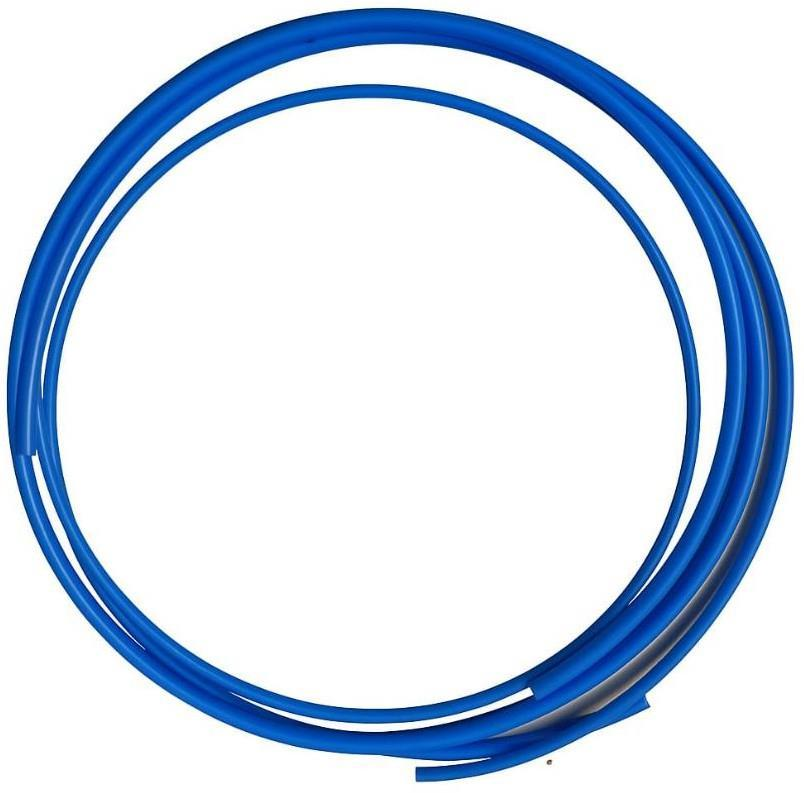
\includegraphics[width=65mm]{figures/fig4_water_supply_pipe.jpg}
\end{center}

\noindent
\begin{spacing}{1.2}
{\fontsize{10.2}{14.5}\selectfont
A flexible blue plastic pipe is used in the system to connect the cold storage water tank with the copper receiver tube. This pipe serves as the main water supply line and ensures a smooth, continuous flow of water from the tank to the receiver during operation.\\[3mm]
\textbf{Material and Function:}
\begin{itemize}[leftmargin=8mm, itemsep=1.5mm, label=\textbullet]
  \item The pipe is made of high-density polyethylene (HDPE), which is lightweight, durable, and resistant to heat and corrosion.
  \item It is capable of withstanding moderate pressure and temperature, making it suitable for small scale solar heating systems.
  \item The inner surface is smooth, allowing easy water flow with minimal frictional losses.
  \item Its blue color helps in identifying it as the cold-water line, preventing confusion with the hot-water outlet.
\end{itemize}
\vspace{2mm}
\textbf{Role in the Project:}
\begin{itemize}[leftmargin=8mm, itemsep=1.5mm, label=\textbullet]
  \item Carries water from the pre-heating storage tank to the copper receiver.
  \item Maintains a constant water level and flow rate in the heating section.
  \item Improves system performance by ensuring that no air pockets or leaks occur.
  \item Flexible enough to accommodate small movements in the solar tracking assembly.
\end{itemize}
}
\end{spacing}
\clearpage
